\chapter{Framework for analytical model}
\label{ch:basics}

\section{Theory of superconductivity}

The discovery of the isotope effect in 1950 revealed that not only lattice electrons but rather the whole lattice determines the superconducting properties of a solid. Experiments measuring the critical temperature $T_c$ of different mercury isotopes showed that indeed, there is a relation between the isotope mass and $T_c$. Herbert Fr\"olich was then the first to introduce a new concept to explain superconductivity. He showed that a phonon-intermediated interaction between electrons and the lattice could lead to an attractive long-range interaction of electrons in the lattice. Figuratively speaking, an electron passing through the crystal lattice will polarize it by attracting the positive ions. It leaves a deformed lattice, which will then attract a second electron. An effective attractive interaction between these two electrons is created. % – they form a Cooper pair. 
In 1956, Cooper showed that the electronic ground state, the Fermi sea at $T = 0$, is unstable if a weak attractive interaction is taken into account. This layed the foundation of the BCS theory \cite{Bardeen1957}, the first microscopic theory after the discovery in 1911 by Heike Kammerlingh Onnes. 

%TODO maybe include picture that explains, why opposite k vectors
%Cooper instability

\subsection*{Formulas needed}
Hamiltonian:
\begin{align}
H &= H_0 + H_1 \label{eq:H}\\
H_0 &= \sum_{\mathbf{k}, \sigma} \xi_{\mathbf{k}} c^{\dagger}_{\mathbf{k} \sigma }c_{\mathbf{k} \sigma }  \label{eq:H0}\\
H_1 &= \frac{1}{N} \sum_{\mathbf{k}, \mathbf{k'}} V_\mathbf{{\mathbf{k}, \mathbf{k'}}} c^{\dagger}_{\mathbf{k} \uparrow }c^{\dagger}_{- \mathbf{k} \downarrow}   c_{- \mathbf{k'} \downarrow} c_{\mathbf{k'} \uparrow} \label{eq:H1}
\end{align}
The operators $c^\dagger_{\mathbf{k}, \sigma} , c_{\mathbf{k}, \sigma}$ are fermion operators that create or annihilate an electron with momentum $\mathbf{k}$ and spin $\sigma$. The first term in the Hamiltonian $H$ is the unperturbed electron Hamiltonian $H_0$ with parabolic energy dispersion $\xi_{\mathbf{k}}$. The  second term is the interaction Hamiltonian $H_1$, expressing the scattering of two electrons from $(- \mathbf{k'} \downarrow,  \mathbf{k'} \uparrow)$ to $(\mathbf{k} \uparrow , - \mathbf{k} \downarrow)$. The interaction potential $V_\mathbf{{\mathbf{k}, \mathbf{k'}}}$ exchanges the scattering for electrons with energy $|\xi_\mathbf{k}| \lesssim \hbar \omega_D$.
%TODO check!
The Hamiltonian in eq. (\ref{eq:H}) can be simplified by doing a mean-field approximation. In this approximation, an operator $A$ is expressed by a sum of its statistical mean $\braket{A}$ and small statistical fluctuations $\delta A$. Since the fluctuations are assumed to be small, terms with $\mathcal{O}((\delta A)^2)$ can be neglected.
\begin{align}
A &= \langle A \rangle + \delta A, \quad B = \langle B \rangle + \delta B  \nonumber \\
A B &= \langle A \rangle  \langle B \rangle  + \langle A \rangle  \delta B +  \langle B \rangle \delta A + \underbrace{\delta A \delta B}_{\approx 0}\label{eq:meanfield-der}
\end{align}
Using $\delta A = A - \langle A \rangle$ and inserting this back into eq. (\ref{eq:meanfield-der}) leads to
\begin{equation}
AB = \langle A \rangle B + \langle B \rangle A - \langle A \rangle \langle B \rangle.\label{eq:meanfield-ab}
\end{equation}
This approximation is applied to the interaction part $H_1$ in eq. (\ref{eq:H1}), replacing
\begin{equation}
A = c^{\dagger}_{\mathbf{k} \uparrow }c^{\dagger}_{- \mathbf{k} \downarrow}, \quad B =  c_{- \mathbf{k'} \downarrow} c_{\mathbf{k'} \uparrow} .
\end{equation}
The result is the BCS-Hamiltonian
\begin{equation}
H_{\text{BCS}} = \sum_{\mathbf{k}, \sigma} \xi_{\mathbf{k}} c^{\dagger}_{\mathbf{k} \sigma }c_{\mathbf{k} \sigma }    -  \sum_{\mathbf{k}} \Delta_{\mathbf{k}}^* c_{-\mathbf{k}, \downarrow} c_{\mathbf{k}, \uparrow}  - \sum_{\mathbf{k}} \Delta_{\mathbf{k}}  c^{\dagger}_{\mathbf{k} \uparrow} c^{\dagger}_{- \mathbf{k} \downarrow} + \text{const.}\label{eq:H-BCS}
\end{equation}
where 
\begin{eqnarray}
\Delta_{\mathbf{k}} &:=& - \frac{1}{N} \sum_{\mathbf{k'}} V_\mathbf{{\mathbf{k} \mathbf{k'}}} \langle c_{-\mathbf{k'}, \downarrow} c_{\mathbf{k'} \uparrow} \rangle \\
\Delta_{\mathbf{k}}^* &:=& - \frac{1}{N} \sum_{\mathbf{k'}} V_\mathbf{{\mathbf{k}, \mathbf{k'}}}  \langle  c^{\dagger}_{\mathbf{k'} \uparrow} c^{\dagger}_{- \mathbf{k'} \downarrow} \rangle
\end{eqnarray}
%TODO why is this the pair potential?
The BCS-Hamiltonian in eq. (\ref{eq:H-BCS}) can be diagonalized using the Bogoliubov transformation. The aim is to express the Hamiltonian in the basis of new fermion operators. These new operators will describe quasiparticles, which are a linear combination of $c^\dagger_{\mathbf{k}, \sigma}$ and $c_{\mathbf{k}, \sigma}$.
\begin{equation}
\begin{pmatrix}
\gamma_{\mathbf{k} \uparrow} \\ \gamma^{\dagger}_{-\mathbf{k} \downarrow}  
\end{pmatrix} = \begin{pmatrix}
u^*_{\mathbf{k} } & -v_{\mathbf{k} } \\
v^*_{\mathbf{k} }  & u_{\mathbf{k} } 
\end{pmatrix} 
\begin{pmatrix}
c_{\mathbf{k} \uparrow} \\ c^{\dagger}_{-\mathbf{k} \downarrow}  
\end{pmatrix}
\end{equation}\label{eq:bogol-trans}
Evaluating the fermion anticommutation relation using the transformation above yields
\begin{equation}
\left\{ \gamma_{\mathbf{k} \uparrow}, \gamma^{\dagger}_{\mathbf{k} \uparrow}  \right\}  = \dots = |u_{\mathbf{k}}|^2 | + v_{\mathbf{k}}|^2 \stackrel{!}{=} 1
\end{equation}
and will lead to the inverse transformation of eq. (\ref{eq:bogol-trans}). Inserting the inverse transformation into the BCS-Hamiltonian in eq.(\ref{eq:H-BCS}) will give the coefficients $u_{\mathbf{k}}$, $v_{\mathbf{k}}$ from eq. (\ref{eq:bogol-trans}) and finally yield to the diagonalized form of the BCS-Hamiltonian
\begin{eqnarray}
H_{\text{BCS}} &=&  \sum_{ \mathbf{k} \sigma } E_{ \mathbf{k} } \gamma^{\dagger}_{\mathbf{k} \sigma } \gamma_{\mathbf{k} \sigma }\\
E_{\mathbf{k}} &:=&  \sqrt{\xi^2_{\mathbf{k}}  + |\Delta_{\mathbf{k}}|^2 }
\end{eqnarray}
%\begin{figure}
%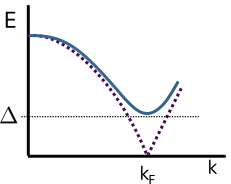
\includegraphics[width=\textwidth]{bcs-spectrum}
%\end{figure}
%TODO below:
\textbf{interpretation as holes, etc \\
plots of particle and hole exitation (dispersion relation with gap)\\
metion fermi surface and so on} \\

\subsection*{Bogoliubov de Gennes Hamiltonian}
%Motivation for BdG: Describing inhomogneous systems, example Josephson junctions --> need for a microsopic theory for inhomogenous systems. 
%Idea: make BCS- mean field hamiltonian spatially dependent. 
The ansatz for the BCS ground state used by Bardeen, Cooper and Schrieffer is based on the concept of Cooper pairs. It is a direct consequence of the instability in the ground state through the attractive interaction. The BCS theory proposes a BCS ground state built on eigenstates of the single-particle Hamiltonian $H_0$ from eq. (\ref{eq:H0}), leading to a ground state that consists of a linear combination of pair states. %TODO check!
\begin{eqnarray}
\ket{\psi_\text{BCS}} &=& \prod_{ \mathbf{k} } (u_\mathbf{k} + v_\mathbf{k} c^{\dagger}_{ \mathbf{k} \uparrow } c^{\dagger}_{ - \mathbf{k} \downarrow }) \ket{\text{vac}} \\
H_\text{BCS} \ket{\psi_\text{BCS}} &=& E_\text{BCS} \ket{\psi_\text{BCS}}  
\end{eqnarray}
In most cases however, a more realistic set-up or inhomogeneous system cannot be described in terms of eigenfunctions of $H_0$. With a vector potential $\mathbf{A} \neq 0$, for example, time reversal symmetry is not given any more. %TODO Überleitung (“In the general case”)
The characteristic length scale is the superconducting coherence length $\xi_0$. If a system is varying slowly over a length scale $l \approx \xi_0$, a spatially dependent, more general Hamiltonian is needed. 
In order to find an adequate expression for such a spatially dependent Hamiltonian, the following spinor is introduced
\begin{equation}
\ket{\Psi_\mathbf{k}} = \begin{pmatrix}
| \Psi_\mathbf{k_1} \rangle \\ | \Psi_\mathbf{k_2} \rangle
\end{pmatrix} := \begin{pmatrix}
c^{\dagger}_{\mathbf{k}, \uparrow} \\ c_{- \mathbf{k}, \downarrow}
\end{pmatrix} \ket{\psi_\text{BCS}} \label{eq:spinor}
\end{equation}
In this basis $\left\{| \Psi_\mathbf{k_1} \rangle, | \Psi_\mathbf{k_2} \rangle \right\}$, the Hamiltonian is (and this is the Bogoliubov de Gennes Hamiltonian with energies relative to $E_\mathbf{k}$):
\begin{equation}
H_\text{BdG}\left(\mathbf{k} \right) = \begin{pmatrix}
\xi_\mathbf{k} &  - \Delta_\mathbf{k}\\
- \Delta^*_\mathbf{k} & - \xi_\mathbf{k}
\end{pmatrix} \label{eq:H-BdG}
\end{equation}
%For this, the commutation relation for $H_\text{BCS}$ and $c^\dagger_{\mathbf{k}, \uparrow}$, $c_{- \mathbf{k}, \downarrow}$ have been used.
This Hamiltonian form eq. (\ref{eq:H-BdG}) has the eigenvalues
\begin{equation}
 \pm E_\mathbf{k} = \pm \sqrt{\xi_\mathbf{k}^2 + |\Delta_\mathbf{k}|^2  }.
\end{equation}
%Include eigenstates?
To finally arrive at the spatially dependent form of eg. (\ref{eq:H-BdG}), the Hamiltonian is Fourier-transformed.
\begin{eqnarray}
H_\text{BdG} \left( \mathbf{r} \right) &:=& \frac{1}{N} \sum_\mathbf{k} e^{i \mathbf{k \cdot r}} H_\text{BdG}\left( \mathbf{k} \right) \\
&=& \begin{pmatrix}
H_0\left( \mathbf{r} \right)  &  - \Delta \left( \mathbf{r} \right) \\
- \Delta^* \left( \mathbf{r} \right)  & - H_0 \left( \mathbf{r} \right) 
\end{pmatrix} \label{eq:H-BdG-r}
\end{eqnarray}
$H_0 \left( \mathbf{r} \right) $ is the free Hamiltonian. Corresponding Schr\"odinger equaions are called BdG-equations:
\begin{eqnarray}
H_\text{BdG} \left( \mathbf{r} \right) \Psi\left( \mathbf{r} \right) &=& E \Psi\left( \mathbf{r} \right)\label{eq:BdG-eq} \\
\Psi\left( \mathbf{r} \right)  &=& \begin{pmatrix}
\Psi_1\left( \mathbf{r} \right) \\ \Psi_2\left( \mathbf{r} \right) 
\end{pmatrix}\label{eq:BdG-spinor}
\end{eqnarray}

\section{Andreev reflection- NS interface}\label{sec:NS}

Now that the principles of BCS theory have been established, the physical effects at the interface between a superconductor and a normal are to be outlined.\\
The most important detail when modelling the interface between a superconductor and a normal metal is the superconducting order parameter $\Delta \left( \mathbf{r} \right)$. It is present in the superconducting region and zero in a normal metal. To keep the model as simple as possible, a step-like behaviour is assumed. This means that for an interface placed at $x=0$, the superconducting order parameter becomes a function of $x$ and can be written as
\begin{equation}
\Delta \left( x \right) = \theta \left(x \right)\label{eq:delta }
\end{equation}.
How does this model differ from a quantum mechanical step potential set-up? The formalism is virtually identical, but there is a subtle and important difference in the results. In the normal region, there are electrons, whereas in the superconducting regions, there is a condensate of Cooper pairs. A normal electron can be reflected at the interface as a hole and an additional Cooper pair can be created in the superconducting region.\\
By solving the Bogoliubov-de-Gennes equation in (\ref{eq:BdG-eq}), this picture becomes clearer.  This equation needs to be solved both for the normal and the superconducting region. When treating this problem quantum-mechanically, energies below and above the gap need to be considered independently. The resulting wave functions have to be continuous at the interface. Depending on the region, the gap parameter in the Hamiltonian in eq. (\ref{eq:H-BdG-r}) is either zero or $\Delta_0$.

\subsection*{Semi-classical approximation: Andreev equations}

In case of the NS interface, the gap parameter varies slowly over scales of $k_F$, and it may vary over scales of the coherence length $\xi_0$. Because $k_F$ is a good length scale for this problem, the equations above can be simplified:
\begin{equation}
\begin{pmatrix} u \\ v \end{pmatrix} = e^{i \mathbf{k_F} \mathbf{r} } \begin{pmatrix} U (x) \\ V(x) \end{pmatrix}.
\end{equation}
Since $U(x)$ and $V(x)$ vary slowly over distances of order $k_F^{-1}$, the second derivative can be neglected. This is the semi-classical approximation, which then leads to the Andreev equations
\begin{eqnarray}
- i \hbar \mathbf{v}_F \nabla U + \Delta V &=& \epsilon U \\
 i \hbar \mathbf{v}_F \nabla V + \Delta^* U &=& \epsilon V.
\end{eqnarray}
These equations are significantly easier to handle than the BdG-equations, since they describe a first-order problem.
\newline
\newline
Consider an incoming particle from the left half-space $x < 0 $, travelling towards the superconducting interface at $x=0$, assuming that both the normal region and the superconductor have the same Fermi velocity $k_F^{-1}$. The one-dimensional Andreev equations for the NS interface read
\begin{eqnarray}
- i \hbar v_{F, x} \frac{d}{dx} U + \Delta(x) V &=& \epsilon U \\
 i \hbar v_{F, x} \frac{d}{dx} V + \Delta^*(x) U &=& \epsilon V.
\end{eqnarray}

\subsubsection*{Solution for the normal region}
In the normal region (for $x < 0$) the superconducting gap parameter decreases to zero on a length scale shorter than $\xi$. Therefore, the step-like approximation from eq. (\ref{eq:delta }) holds. In the normal region, 
the coefficients $U(x)$ and $V(x)$ are independent. The ansatz contains an incident wave with unity amplitude and a reflected hole with amplitude $a$. 
\begin{equation}
\begin{pmatrix} U(x) \\ V(x) \end{pmatrix}_N = e^{i k_N x } \begin{pmatrix} 1 \\ 0 \end{pmatrix} + a e^{-i k_N x } \begin{pmatrix} 0 \\ 1 \end{pmatrix} 
\end{equation}
where 
\begin{equation}
k_n = \frac{\epsilon}{\hbar v_x}
\end{equation}
And therefore the solution to the Andreev reflection is ($|\mathbf{k}| = k_F$)
\begin{eqnarray}
\begin{pmatrix} u \\v \end{pmatrix} &=& e^{i\mathbf{k} \cdot \mathbf{r}} \begin{pmatrix} U(x) \\V(x) \end{pmatrix}\\
&=& e^{i\mathbf{q}_+ \cdot \mathbf{r}} \begin{pmatrix} 1 \\ 0\end{pmatrix} + a e^{i\mathbf{q}_- \cdot \mathbf{r}} \begin{pmatrix} 0 \\ 1\end{pmatrix},
\end{eqnarray}
with
\begin{equation}
\mathbf{q}_\pm =  \left( k \pm \frac{\epsilon}{\hbar v_F} \right) \hat{\mathbf{k}} 
\end{equation}

\subsubsection*{Solution in the superconducting region}
In the superconducting region, the solution for the wave function has the form
\begin{equation}
\begin{pmatrix} U(x) \\ V(x) \end{pmatrix}_S = c e^{i k_S x } \begin{pmatrix} U_0 \\ V_0 \end{pmatrix},
\end{equation}
where $c$ is the amplitude and $k_S$ is the wave vector. The expression for $k_S$ depends on the energy of the incoming particle, which can be either \emph{above} or \emph{below} the gap.\newline \newline
For high energies \emph{above} the gap,  $E > |\Delta|$ , the wave vector is
\begin{equation}
k_S = \frac{\sqrt{\epsilon^2 - \Delta^2}}{\hbar v_x}
\end{equation}
The coherence factor $U_0$, $V_0$ can be found by solving the BdG equations within the BCS framework. Matching the boundary conditions at the interface yields
\begin{equation}
a = \frac{V_0}{U_0}, \quad c = \frac{1}{U_0}.
\end{equation}
In this solution, the incoming electron has the momentum 
\begin{equation}
q  = k_F + \frac{\epsilon}{\hbar v_F} \quad \rightarrow \epsilon(q) = \hbar v_F \left( q - k_F \right)
\end{equation}
with a positive group velocity $v_g = v_F$, whereas the reflected hole has the momentum
\begin{equation}
q  = k_F - \frac{\epsilon}{\hbar v_F} \quad \rightarrow \epsilon(q) = \hbar v_F \left( k_F - q \right)
\end{equation} 
with negative group velocity $v_g = - v_F$. \\
By calculating the change in the momentum one finds the trajectory of the reflected hole to coincide with the trajectory of the incoming electron. The change in momentum is
\begin{equation}
\Delta p_x = \left( \hbar k_x - \frac{\epsilon}{v_x} \right) -  \left( \hbar k_x + \frac{\epsilon}{v_x} \right) = - \frac{2 e }{v_x}
\end{equation}
$p_y$, $p_z$ are conserved, $\Delta p_x$ is small, therefore the trajectory of the reflected hole is almost the same as the trajectory of the incoming electron.
%TODO figure!
%Probabilities: 
%\begin{equation}
%|a|^2 + (U_0^2- V_0^2)|c|^2 = 1
%\end{equation}
\newline
\newline
For energies \emph{below} the gap, $\epsilon < |\Delta |$, there are no states available inside the gap, therefore the wave function decays inside the superconductor. 
\begin{equation}
\tilde{k}_S= \frac{\sqrt{\Delta^2 - \epsilon^2 }}{\hbar v_x}.
\end{equation}
The wave function is
\begin{equation}
\begin{pmatrix} U(x) \\ V(x) \end{pmatrix}_S = c e^{- \tilde{k_S} x } \begin{pmatrix} U_0 \\ V_0 \end{pmatrix}.
\end{equation}
For sub-gap energies, the amplitudes of the normal wave functions are slightly modified:
\begin{equation}
a = \frac{\tilde{V_0}}{\tilde{U_0}}, \quad c = \frac{1}{\tilde{U_0}}
\end{equation}
and 
\begin{equation}
\tilde{U_0} = \frac{1}{\sqrt{2}} \left( 1 + i \frac{\sqrt{|\Delta|^2 - \epsilon^2}}{\epsilon} \right), \quad \tilde{V_0} = \frac{1}{\sqrt{2}} \left( 1 - i \frac{\sqrt{|\Delta|^2 - \epsilon^2}}{\epsilon} \right).
\end{equation}
In this case, it holds that
\begin{equation}
|a|^2 = 1
\end{equation}
In other words, there are no transmitted particles and all particles are Andreev reflected.

\section{Theory of SNS junction}
So far, only NS interfaces have been considered. The same procedure can be applied to superconductor - normal metal - superconductor (SNS) junctions: A sandwich structure of a superconductor on the left side, a normal region in the middle and a superconductor on the right side. At both interfaces, a particle can be Andreev-reflected.
Each time an electron is Andreev reflected at the right side and a hole travels back, a cooper pair is induced into the right superconductor. In the same manner, a cooper pair is stolen from the left superconductor when the hole is Andreev reflected as an electron. As an overall consequence, a supercurrent through the SNS junction can be observed. This process leads to localized electrons with bound states, the so called Andreev bound states. \\

A SNS junction with normal region at $|x| < W/2$, the right superconductor at $x > + W/2$ and the left superconductor at $x < -W/2$ is considered. The electrons in both superconducting regions and in the normal metal have the same Fermi velocity and there are no insulating barriers between them. This means that $W$  is smaller than the electron mean free path. For short $W$ this implies that the mean free path is larger than the superconducting coherence length (?). The phase difference between the superconductors is $\chi$, so the right supercondctor has phase $\chi/2$ and the left has $-\chi/2$. 
The semi classical approximation is used and a wave function with the form
\begin{equation}
\begin{pmatrix} u \\ v \end{pmatrix} = e^{i \mathbf{k_F} \mathbf{r} } \begin{pmatrix} U (x) \\ V(x) \end{pmatrix}.
\end{equation}
is needed.\newline
In the normal region, it holds that 
\begin{equation}
\begin{pmatrix} U(x) \\ V(x) \end{pmatrix}_N = A\cdot \left[ e^{i k_N x } \begin{pmatrix} 1 \\ 0 \end{pmatrix} + a e^{-i k_N x } \begin{pmatrix} 0 \\ 1 \end{pmatrix} \right], \quad k_N = \frac{\epsilon}{\hbar v_x}.
\end{equation}
Assuming that $k_x > 0$, the wave function in the right superconductor ($x > W/2$) is
\begin{equation}
\begin{pmatrix} U(x) \\ V(x) \end{pmatrix}_R = d_1 e^{ - \tilde{k}_S x } \begin{pmatrix} \tilde{U} e^{i \chi/4} \\ \tilde{V} e^{-i \chi/4} \end{pmatrix}, \quad \tilde{k}_S  = \frac{\sqrt{|\Delta|^2 - \epsilon^2 }}{\hbar |v_x|}.
\end{equation}
For the left superconductor, the wave function is
\begin{equation}
\begin{pmatrix} U(x) \\ V(x) \end{pmatrix}_L = d_1' e^{ \tilde{k}_S x } \begin{pmatrix} \tilde{V} e^{-i \chi / 4}\\ \tilde{U} e^{i \chi / 4} \end{pmatrix}.
\end{equation}
Applying the continuity condition at the interfaces leads to
\begin{eqnarray}
a e^{-i k_n W} &=& \frac{\tilde{V}}{\tilde{U}} e^{-i \chi /2}  \\
a e^{i k_n W} &=& \frac{\tilde{U}}{\tilde{V}} e^{i \chi /2}.
\end{eqnarray}
Combining these equations, we find
\begin{equation}
e^{2i ( k_N W - \chi /2 )}  = \frac{\epsilon + i \sqrt{|\Delta|^2 - \epsilon^2 }}{ \epsilon - i \sqrt{|\Delta|^2 - \epsilon^2 } } \label{eq:energy-exp}.
\end{equation}
To simplify this expression, one can introduce 
\begin{equation}
\sin \alpha := \frac{\epsilon}{|\Delta|}, \quad - \pi / 2 < \alpha < \pi / 2\label{eq:sinalpha}
\end{equation}
Using eq. (\ref{eq:sinalpha}), one can rewrite the right hand side of eq. (\ref{eq:energy-exp}) in terms of trigonometric functions and gets
\begin{equation}
e^{2i ( k_N W - \chi /2 )} = e^{-2i \alpha + i \pi},
\end{equation}
which then leads to
\begin{equation}
\epsilon = \frac{\hbar v_x}{W} \left( \pi \left(l + \frac{1}{2} \right) - \arcsin \frac{\epsilon}{|\Delta|} + \frac{\chi}{2} \right).
\end{equation}
%TODO short summary, what has been done up to this point?
If $k_x < 0 $, it holds that
\begin{equation}
\begin{pmatrix} U(x) \\ V(x) \end{pmatrix}_R = d_2 e^{ - \tilde{k}_S x } \begin{pmatrix} \tilde{V} e^{i \chi/4} \\ \tilde{U} e^{-i \chi/4} \end{pmatrix}
\end{equation}
For the left superconductor, the wave function is
\begin{equation}
\begin{pmatrix} U(x) \\ V(x) \end{pmatrix}_L = d_2' e^{ \tilde{k}_S x } \begin{pmatrix} \tilde{U} e^{-i \chi / 4}\\ \tilde{V} e^{i \chi / 4} \end{pmatrix}
\end{equation}
An analogous calculation leads to
\begin{equation}
\epsilon = - \frac{\hbar |v_x|}{W} \left( \pi \left(l - \frac{1}{2} \right) + \arcsin \frac{\epsilon}{|\Delta|} + \frac{\chi}{2} \right)
\end{equation}
The final result for the spectrum is
\begin{equation}
\epsilon = \pm \frac{\hbar |v_x|}{W} \left( \pi \left(l \pm \frac{1}{2} \right) \mp \arcsin \frac{\epsilon}{|\Delta|} + \frac{\chi}{2} \right)
\end{equation}
The upper sign is equivalent to $k_x > 0$ and the lower sign is equivalent to $k_x  <0 $.\\
Normalizing the wave functions yields the coefficient
\begin{equation}
|A|^2 = \frac{1}{2(W+ k_S^{-1})} = \frac{1}{2} \frac{\sqrt{|\Delta|^2 - \epsilon^2}}{\hbar |v_x| + W \sqrt{|\Delta|^2 - \epsilon^2}}.
\end{equation}
%TODO maybe a bit more how |A|^2 is calculated?
\subsubsection*{Limit of short junction}

For junctions with small width $W$,
\begin{equation}
W \ll \frac{\hbar v_x }{|\Delta|}, \quad \xi \ll W
\end{equation}
where $\xi \sim \hbar v_F / |\Delta|$ is the coherence length. Then, in eq. (\ref{eq:energy-exp}) the term with $e^{2i k_n W} \approx 1$ and the spectrum becomes
\begin{equation}
\epsilon = \mp \cos \frac{\chi}{2}, \quad 0 < \chi < \pi
\end{equation}

\subsubsection*{Limit of long junction}

Long junction, $W \gg \xi_0$, it hold that 
\begin{equation}
W \gg \frac{\hbar |v_x|}{|\Delta|} 
\end{equation} 
then the spectrum is (because $\arcsin \frac{\epsilon}{|\Delta|}$ can be neglected
\begin{equation}
\epsilon = \pm \frac{\hbar |v_x|}{W}\left(\frac{\chi}{2} - \frac{\pi}{2} \right) + \frac{l \pi \hbar |v_x|}{W} 
\end{equation}

\section{Supercurrent through the SNS junction}
Having established the normal wave functions for SNS junctions, the quantum-mechanical current can be calculated.
\begin{equation}
\mathbf{j} = \frac{e}{m} \left[ f_n u_n^* \left( \mathbf{r} \right) \left( - i \hbar \nabla - \frac{e}{c} \mathbf{A} \right) u_n\left( \mathbf{r} \right) + \left(1-f_n\right) v_n\left( \mathbf{r} \right) \left( -i \hbar \nabla - \frac{e}{c} \mathbf{A} \right) v_n^*\left( \mathbf{r} \right) + \text{c.c.} \right] \label{eq:current-qm}
\end{equation}
$n$ labels quantum states, $f_n$ is the corresponding Fermi distribution.
As a simplification, $\mathbf{A} = 0$ is considered. For evaluating eq. (\ref{eq:current-qm}), the normal wave functions are used. In the semi-classical approximation, only the derivatives of the rapidly varying functions $e^{i\mathbf{k r}}$ contribute to the current.
\begin{eqnarray}
\mathbf{j} &=& - i \hbar  \frac{e}{m} \left[ f_n u_n^* \left( \mathbf{r} \right) \nabla  u_n \left( \mathbf{r} \right) + \left(1-f_n\right) v_n\left( \mathbf{r} \right) \nabla v_n^*\left( \mathbf{r} \right) + \text{c.c.} \right]\\
I_x &=& - \frac{e}{\hbar} \sum_n \left(1- 2 f_n \right) \frac{\hbar v_x \sqrt{|\Delta^2| - \epsilon_n^2}}{\hbar v_x + W \sqrt{|\Delta|^2 -\epsilon^2}}
\end{eqnarray}

\section{Specular Andreev reflection, graphene specifics}
An unusual form of Andreev reflection has been found on graphene - superconductor interfaces %TODO cite.
In the previously discussed Andreev retro reflection, the electron and the reflected hole both lie in the conductance band. In more exotic materials, like  single layer graphene (SLG), the reflected hole undergoes a transition to the valence band. In this case, the reflection angle is a function of $E_F$, and for $E_F = 0$, the reflection is specular.
For graphene, the single particle Hamiltonian is the Dirac Hamiltonian
\begin{eqnarray}
H &=& \begin{pmatrix}
H_+ & 0 \\
0 & H_- 
\end{pmatrix} \\
H_\pm &=& i \hbar \left( \sigma_x \delta_x \pm \sigma_y \delta_y \right) + U
\end{eqnarray}
This modifies the BdG-equation and leads to interesting results when calculating the Andreev reflection amplitude. 
\begin{equation}
\begin{pmatrix}
H_\pm + E_F & \Delta \\
\Delta^* & E_F - H_\pm 
\end{pmatrix} \begin{pmatrix}
u \\ v \end{pmatrix} = \epsilon \begin{pmatrix} u \\v \end{pmatrix} \label{eq:dirac-hamiltonian}
\end{equation}
The electron spinor has two components $\begin{pmatrix} u_1, u_2\end{pmatrix} = \begin{pmatrix} \Psi_{A+}, \Psi_{B+} \end{pmatrix}$, and the hole spinor is $\begin{pmatrix} v_1, v_2\end{pmatrix} = \begin{pmatrix} \Psi^{*}_{A-} - \Psi^{*}_{B-} \end{pmatrix}$.
The Hamiltonian from eq. (\ref{eq:dirac-hamiltonian}) leads to the energy spectrum
\begin{equation}
\epsilon = \sqrt{|\Delta|^2 + \left( E_F - U \pm \hbar v |\mathbf{k}|\right) ^2}, \quad |\mathbf{k}| = \sqrt{k_x^2 + k_y^2}.
\end{equation}
The dispersion relation has four solutions for $\mathbf{k}$. Since $k_y$ and $\epsilon$ are preserved, a general scattering state is a superposition of these four solutions for $k_x$. The derivative $\hbar^{-1} d\epsilon / d k_x$, the velocity in x direction, gives two solutions with negative slope and two with positive slope. The two solutions for $k_x$ which lead to a positive velocity consist of one electron excitation ($v=0$) and one hole excitation ($u=0$). 
From the BCS mean field theory it is known that $\Delta_0 \ll E_F + U_0$, or equivalently $\xi = \hbar v /\Delta_0 \gg \lambda_F^{sc}$, the Fermi wave length in the superconductor. The magnitude of $\xi$ and the Fermi wave length in the normal region, $\lambda_F^{n}$, is not constrained.
%TODO pretty picture
%TODO 
Look at the solution for two different regimes:\\
$\mathbf{\epsilon < E_F}$:  the reflected hole is in an empty state in the conduction band. A conduction band hole moves opposite to its wave vector, so $v_y$, $v_x$ change sign $\rightarrow$ Andreev retro reflection \\
$\mathbf{\epsilon > E_F}$: reflected hole is in an empty state in the valence band. Valence band hole moves into same direction as its wave vector, so $v_y$ remains the same, $v_x$ changes sign $\rightarrow$ Andreev specular reflection. \\
At energies $\epsilon \lesssim \Delta_0$, retro reflection is the dominant process for $E_F \gg \Delta_0$, and specular reflection dominates if $E_F \ll \Delta_0$.
The probability of the electron--hole conversion can be calculated by solving the Dirac-BdG equations matching boundary conditions at the interface. The resulting reflection amplitude for electron to electron (what) is denoted with $r\left( \epsilon, \alpha\right)$, where $\alpha$ is the angle of incidence (angle between incoming vector and x-axis). The Andreev reflection amplitude for electron to hole is $r_A \left( \epsilon, \alpha \right)$. The difference of the NS interface for graphene and a superconductor is that the Andreev reflection amplitude is unity for $\alpha = 0$, whereas in a normal NS interface Andreev reflection is suppressed for all angles. 
The fact that the reflection at the interface always converses the charge is a consequence of the conservation of chirality, meaning the sublattice index. When an electron is Andreev reflected as a hole, the reflected hole moves on the same sublattice, while the reflection without charge conversion would require scattering from one sublattice to the other. (?)

% Specular reflection manifests itself in the differential conductance


%Applying the same methods as above, the 
 
